\documentclass[border=3pt,varwidth]{standalone}
\usepackage{amsmath,amssymb}
\usepackage{tikz}
\usetikzlibrary{arrows.meta,calc,decorations.markings,patterns,positioning,angles,quotes}
\tikzset{
  >=Stealth,
  every node/.style={font=\normalsize},
  wire/.style={line width=0.9pt},
  thinwire/.style={line width=0.6pt},
  fieldline/.style={line width=0.6pt,-{Stealth[length=2.2mm]}},
  axis/.style={line width=0.7pt,-{Stealth[length=2.2mm]}},
  dashedwire/.style={line width=0.9pt,dash pattern=on 3pt off 2pt},
  resistor/.style={line width=0.9pt},
  chargepos/.style={circle,draw,line width=0.8pt,minimum size=5mm,inner sep=0pt},
  dotcharge/.style={circle,fill,inner sep=0pt,minimum size=2.4pt}
}
% Draw a resistor box centered at (x,y) with width w, height h, horizontal
\newcommand{\resbox}[4]{%
  % #1=x #2=y #3=halfwidth #4=label
  \draw[resistor] (#1-#3,#2-0.18) rectangle (#1+#3,#2+0.18);
  \ifx\\#4\\\else\node[above=2pt] at (#1,#2+0.18) {#4};\fi
}
% Battery symbol: long thin line (+) then short thick line (-), centered at (x,y)
\newcommand{\battery}[2]{%
  % #1=x #2=y ; long line left=+, short line right=- by default orientation
  \draw[wire] (#1-0.09,#2-0.32) -- (#1-0.09,#2+0.32);
  \draw[line width=2.6pt] (#1+0.09,#2-0.16) -- (#1+0.09,#2+0.16);
}

\begin{document}
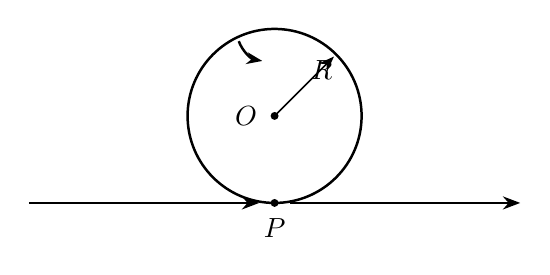
\begin{tikzpicture}[scale=1.3]
  \def\R{0.85}
  \draw[wire] (0,\R) circle (\R);
  \fill (0,\R) circle (1.1pt);
  \node[left=1pt] at (-0.05,\R) {$O$};
  \draw[thinwire,-{Stealth[length=2mm]}] (0,\R) -- (0.58,\R+0.58);
  \node[above right=-2pt] at (0.3,\R+0.3) {$R$};
  % small curved arrow at the top of the loop indicating current direction
  \draw[wire,-{Stealth[length=2mm]}] (-0.35,2*\R-0.12) arc[start angle=200,end angle=260,radius=0.3];
  % straight wire through point P at the bottom of the circle
  \draw[wire,-{Stealth[length=2.2mm]}] (-2.4,0) -- (-0.15,0);
  \draw[wire,-{Stealth[length=2.2mm]}] (0.15,0) -- (2.4,0);
  \fill (0,0) circle (1.1pt);
  \node[below=2pt] at (0,0) {$P$};
\end{tikzpicture}
\end{document}
